%%%%%%%%%%%%%%%%%%%%%%%%%%%%%%%%%%%%%%%%%%%%%%%%%%%%%%%%
%%%%%%%%%%%%%%%%%%%%%%%%%%%%%%%%%%%%%%%%%%%%%%%%%%%%%%%%
\chapter{\pandas}
\label{pandas}

%%%%%%%%%%%%%%%%%%%%%%%%%%%%%%%%%%%%%%%%%%%%%%%%%%%%%%%%
%%%%%%%%%%%%%%%%%%%%%%%%%%%%%%%%%%%%%%%%%%%%%%%%%%%%%%%%
\section{Basic Commands}
\label{pandas:basic}

\begin{lstlisting}[language=Python]
# IO
df = pd.read_csv('file.csv', header=None)
df['col'] = df['col'].astype(int)
df.to_csv('out.csv')

# descriptive commands
df.describe(); df.columns; df.shape;

# aggregation commands
df.sum(); df.cumsum();
df.min(); df.max(); df.idxmin(); df.idxmax();
df.mean(); df.std(); df.median(); df.mode();

# extract all rows from one column
df_y = df.loc[:, ['y']]

# select by value
df_selection = df.loc[( ((df['x'] == x_value) & (df['y'] == y_value)) | (df['z'] > z_value))]

# select by value and assign new value
df.loc[(df['x'] == x_value), 'y'] = y_value

# select with query
df_selection = df.query('x > 0')

# select with isin
df_selection = df.isin({'x': [x_value1, x_value2], 'y': [y_value]})

# select row by index
series = df.iloc[0]

# apply an arbitrary function
def func(x, y):
  return x*np.sin(y)
df['z'] = np.vectorize(func)(df['x'], df['y'])

# iterate through rows
for index, row in df.iterrows():
  x_value = row['x']

# construct from rows
rows_list = []
for nrow in range(nrows):
  rows_list.append({'x':x_value, 'y':y_value})
df = pd.DataFrame(rows_list)
df = df[['x', 'y']]

# rename columns
df = df.rename({'old': 'new'}, axis='columns')

# sort
df = df.sort_values(by=['x', 'y'], ascending=[True, False]).reset_index(drop=True)

# group by, while dropping new count column and duplicates
df = df.groupby(['x', 'y', 'z']).size().to_frame(name = 'count').reset_index().drop(['count'], axis=1).drop_duplicates()

# return duplicate rows
columns_to_check_for_duplicates = ['x', 'y']
df_duplicates = df[df.duplicated(subset=columns_to_check_for_duplicates, keep=False)]

# shuffling
df = df.sample(frac=1., replace=False, random_state=rnd_seed).reset_index(drop=True)

# drop columns
df = df.drop(['col_to_drop1', 'col_to_drop2'], axis=1)

# fill nans, for all columns and per column 
df = df.fillna(0.0)
df = df.fillna(value={'x': x_nan_value, 'z': y_nan_value})
\end{lstlisting}

\clearpage

%%%%%%%%%%%%%%%%%%%%%%%%%%%%%%%%%%%%%%%%%%%%%%%%%%%%%%%%
%%%%%%%%%%%%%%%%%%%%%%%%%%%%%%%%%%%%%%%%%%%%%%%%%%%%%%%%
\section{Joining}
\label{pandas:join}

\noindent See the \href{https://pandas.pydata.org/pandas-docs/stable/user_guide/merging.html}{documentation} and this \href{http://chrisalbon.com/python/data_wrangling/pandas_join_merge_dataframe/}{useful guide}.

\begin{lstlisting}[language=Python]
df = pd.merge(df_l, df_r, left_on='id_left', right_on='id_right', how='left')
\end{lstlisting}

%%%%%%%%%%%%%%%%%%%%%%%%%%%%%%%%%%%%%%%%%%%%%%%%%%%%%%%%
%%%%%%%%%%%%%%%%%%%%%%%%%%%%%%%%%%%%%%%%%%%%%%%%%%%%%%%%
\section{Pivoting}
\label{pandas:pivoting}

\subsubsection{pivot}
\label{pandas:pivoting:pivot}

\noindent \href{http://pandas.pydata.org/pandas-docs/stable/reference/api/pandas.DataFrame.pivot.html}{\texttt{pivot} documentation}.

\begin{lstlisting}[language=Python]
DataFrame.pivot(index=None, columns=None, values=None)
\end{lstlisting}

\begin{figure}[H]
\centering
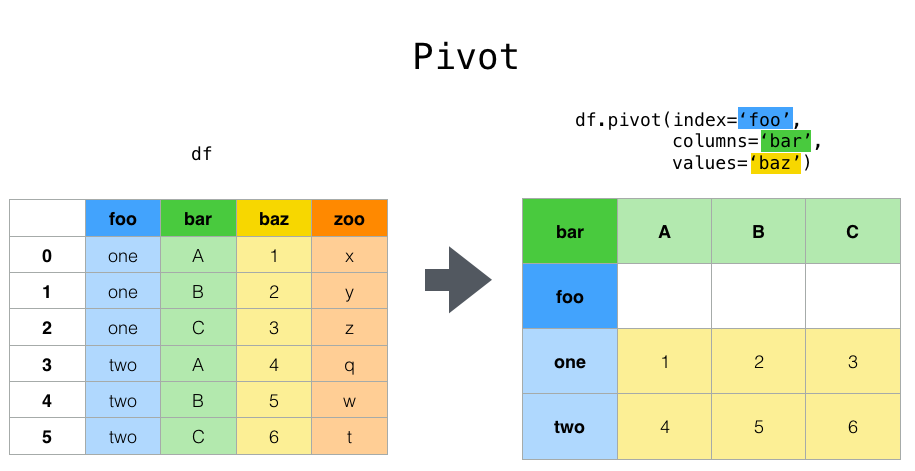
\includegraphics[width=0.85\textwidth]{figures/pandas/reshaping_pivot.png}
\caption{
Example \pandas \texttt{pivot} operation, from the package \href{http://pandas.pydata.org/pandas-docs/stable/user_guide/reshaping.html}{documentation}.
}
\label{fig:pandas:pivot}
\end{figure}

\subsubsection{pivot\_table}
\label{pandas:pivoting:pivot_table}

\noindent \href{https://pandas.pydata.org/pandas-docs/stable/reference/api/pandas.pivot_table.html}{\texttt{pivot\_table} documentation}.

\begin{lstlisting}[language=Python]
pandas.pivot_table(data, values=None, index=None, columns=None, aggfunc='mean', fill_value=None, margins=False, dropna=True, margins_name='All')
\end{lstlisting}

\begin{figure}[H]
\centering
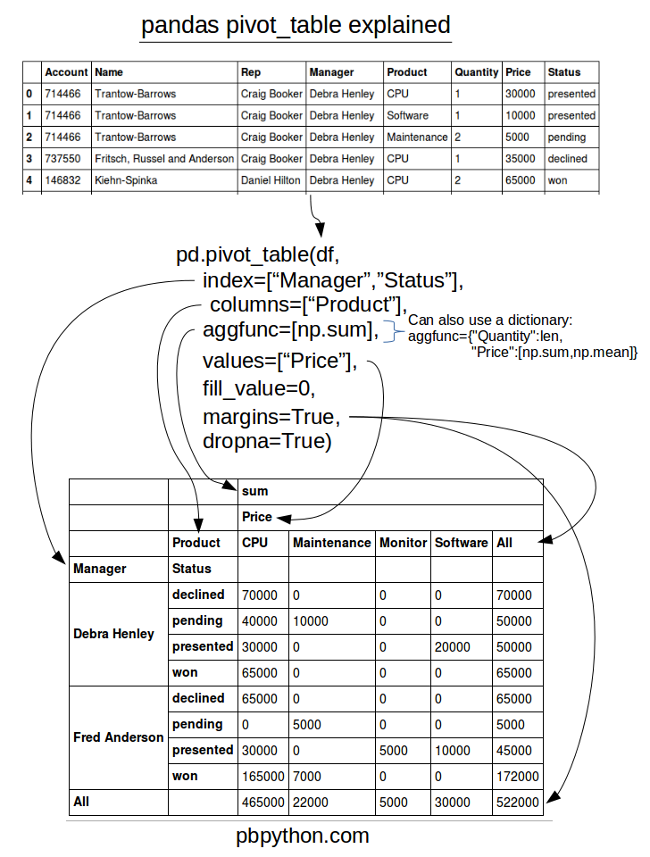
\includegraphics[width=0.95\textwidth]{figures/pandas/pivot-table-datasheet.png}
\caption{
Example \pandas \texttt{pivot\_table} operation, by \href{http://pbpython.com/pandas-pivot-table-explained.html}{Chris Moffitt}.
}
\label{fig:pandas:pivot_table}
\end{figure}
